%% Local proof build of the SAME body.tex, using the standard article class.
%% Purpose: verify the manuscript body compiles (text, maths, tables, figures, citations)
%% on a machine without sn-jnl.cls. This is NOT the submission file -- submit manuscript.tex.
%%
%%   pdflatex proof && bibtex proof && pdflatex proof && pdflatex proof

\documentclass[11pt,a4paper]{article}

\usepackage[T1]{fontenc}
\usepackage[utf8]{inputenc}
\usepackage[margin=2.2cm]{geometry}
\usepackage{graphicx}
\usepackage{booktabs}
\usepackage{rotating}
\usepackage{tabularx}
\usepackage{xltabular}
\usepackage{makecell}
\usepackage{pdflscape}
\usepackage{url}
\usepackage{amsmath}
\usepackage{amssymb}
\usepackage[numbers,sort&compress]{natbib}
\usepackage[htt]{hyphenat}   % allow hyphenation inside \texttt identifiers
\usepackage{hyperref}
% Suppress the coloured link borders. They make a proof look like a working draft, and a
% reviewer reasonably flagged them as a production defect.
\hypersetup{hidelinks}
\setlength{\emergencystretch}{3em}

\graphicspath{{figures/}}
\bibliographystyle{unsrtnat}

% sn-jnl provides \bmhead and \sur/\fnm; stub them so body.tex and the declarations compile here.
\providecommand{\bmhead}[1]{\subsection*{#1}}

\title{QSARena: separating model-library breadth from held-out selection in a leakage-controlled, cross-suite benchmark of molecular property-prediction models}
\author{Scott Coffin (ORCID 0000-0002-7035-1282)\\\small California Office of Environmental Health Hazard Assessment, Sacramento, CA, USA}
\date{\today}

\begin{document}
\maketitle
%% Front matter shared verbatim with manuscript.tex, so this proof shows the COMPLETE paper.
%% An earlier version of this shim omitted these, and a reviewer reasonably read the resulting
%% PDF as lacking a structured abstract, keywords and declarations. Keep these in sync by
%% construction: both files \input the same sources.
\begin{abstract}
\noindent\textbf{Background.} ADMET prediction is dominated by ever-larger pretrained models, whose compute cost and reproducibility limit adoption in academic, regulatory and small laboratories. Recent benchmarks report that added scale rarely translates into accuracy but rarely ask how much of a model's leaderboard standing comes from library breadth and from held-out selection. Neither has been tested across benchmark suites under one fixed, leakage-controlled pipeline.

\textbf{Methods.} QSARena, a code-free notebook and command-line runner, evaluated 31 models on 44 datasets from five suites (22 regression, 22 classification; 1094 model--dataset evaluations) under one fixed configuration without per-dataset tuning, with feature selection nested inside cross-validation.

\textbf{Results.} Nested feature selection cut median cross-validation optimism from 15.9\% to 3.4\%; cross-validation selection then picked the per-dataset winner on 4 datasets and sat a median 7.7\% from the test-selected best. Against published values, estimated top-ten placement fell from 35 to 27 of 37 comparable datasets under cross-validation selection; a matched-candidate-set control attributes 7 of those 8 lost placements to library breadth and 1 to held-out selection. No single family dominated: conventional machine learning won 6 datasets, Chemprop and 3D pretrained models 5 each and TabPFN 3, while ensembles built from these families' out-of-fold predictions (not like-for-like single models) won 22 and were most consistent (within 5\% of best on 84\% of datasets). Ranks are provisional, as some references have documented leakage; a consumer-laptop GPU changed the best single-model score by a median of $+0.5$\%.

\textbf{Conclusions.} Library breadth drives most leaderboard standing; held-out selection still contributes measurable optimism. Added model scale was not required for competitive accuracy; no tuning, installation or specialized hardware is needed. Results derive from a single split and seed, so close margins are provisional.

\textbf{Scientific Contribution.} We report a uniform, leakage-controlled benchmark across five suites (44 datasets, 31 models) under one fixed configuration. We decompose the gap between test-selected and cross-validation-selected standing into library breadth (7 of 37 placements) and held-out selection (1 of 37), an inflation affecting any comparably selected entry but rarely reported. Both protocols share one run and reference set, so the decomposition is less sensitive to reference quality than absolute ranks.

\end{abstract}

\medskip
\noindent\textbf{Keywords:} QSAR, ADMET, AutoML, Molecular property prediction, Benchmarking, Reproducibility, Data leakage, Ensemble learning, Foundation models, Open-source software, Accessibility


\bigskip
\noindent\textbf{Graphical abstract} (submitted separately, 920$\times$300\,px):

\noindent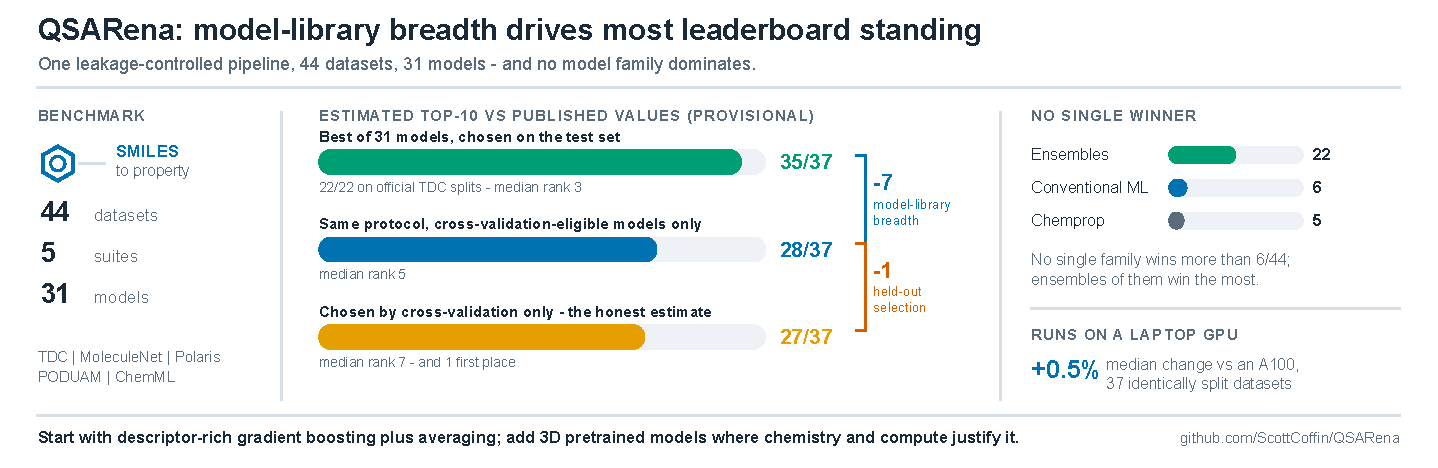
\includegraphics[width=\linewidth]{figures/graphical_abstract.pdf}

\clearpage

%% Shared manuscript body. Included by manuscript.tex (Springer Nature sn-jnl, for submission)
%% and by proof.tex (article class, for local proof compilation). Do not add \documentclass,
%% \begin{document} or front matter here.

\section{Introduction}\label{sec:background}

Unfavourable absorption, distribution, metabolism, excretion and toxicity (ADMET) properties remain among the most consequential causes of failure in drug development. About 90\% of drug candidates that enter clinical testing fail, mainly for lack of clinical efficacy or unmanageable toxicity, with poor drug-like properties, including unfavourable pharmacokinetics, a smaller but material share \cite{sun2022why90}; inappropriate pharmacokinetics and bioavailability fell from roughly 40\% of clinical attrition in the early 1990s to about 10\% by 2000 once the industry adopted routine early ADME profiling \cite{kola2004attrition}. Because experimental ADMET assays are slow, costly and hard to scale, \emph{in silico} prediction of ADMET endpoints from chemical structure has become an indispensable complement to laboratory screening \cite{fu2024admetlab,komura2023trends}.

Standardized public benchmarks have driven much of this progress. MoleculeNet established curated datasets and evaluation protocols for molecular machine learning \cite{wu2018moleculenet}, and the Therapeutics Data Commons (TDC) consolidated a large collection of ADMET datasets into a benchmark group with fixed splits, per-task metrics and a public leaderboard enabling direct comparison \cite{huang2021tdc}. More recent resources such as Polaris have emphasized immutable, standardized benchmarks as a route to reproducible comparison. These resources catalysed rapid methodological progress, but also fostered a leaderboard culture in which incremental gains are pursued through increasingly elaborate architectures.

A prominent expression of this trend is the turn toward large pretrained ``foundation'' models. Graph-based models such as MolE, pretrained on roughly 842 million molecules \cite{mendezlucio2024mole}, and MolGPS, scaled to three billion parameters with the aid of phenomics data \cite{sypetkowski2024molgps}, have established state-of-the-art results on subsets of the TDC ADMET tasks, and parameter-efficient successors such as MiniMol have continued this line of work \cite{klaser2024minimol}. Three-dimensional pretrained models such as Uni-Mol, which learns from conformer geometry rather than 2D topology alone, represent a distinct and comparatively cheap point on this spectrum \cite{zhou2023unimol}. While impressive, the largest of these models require very large pretraining corpora, specialized hardware and substantial engineering expertise, placing them out of practical reach for many of the settings in which ADMET prediction is most needed.

Critically, the assumption that architectural scale translates into superior ADMET prediction is not well supported. In a comprehensive benchmark of twelve representative models, three non-deep and nine deep, Xia et al.\ found that deep models generally fail to outperform non-deep ones, gradient-boosted trees and random forests on molecular fingerprints tending to perform best because tree models suit the non-smooth target functions of molecular property prediction \cite{xia2023understanding}, and a review in the \emph{Annual Review of Biomedical Data Science} found that a substantial and consistent advantage of deep learning over standard machine learning across diverse datasets and properties has not been demonstrated \cite{rodriguezperez2022machine}. Cross-suite studies since have reinforced this picture rather than overturned it: across diverse real-world datasets the best method is dataset-dependent, and engineered features with classical learners often match or exceed deep models \cite{green2023current}; a 2026 systematic survey identifies reproducibility limits in current splitting and evaluation protocols \cite{li2026systematic}; and a large reliability study found that the tabular foundation model TabPFNv2 often generalised better than customized molecular foundation models in few-shot and out-of-distribution settings \cite{zhao2026revisiting}.

These observations are borne out on the TDC leaderboard itself, where gradient boosting on combined fingerprint and descriptor representations remains highly competitive: extreme gradient boosting (ADMETboost) \cite{tian2022admetboost}; CatBoost paired with ECFP, Avalon and ErG fingerprints plus ${\sim}200$ molecular properties, which achieved top-3 performance on 16 of 22 benchmarks (the MapLight submission) \cite{notwell2023admet}; AutoML over descriptor sets (CaliciBoost) \cite{le2025caliciboost}; and automatic feature-combination frameworks built on simple learners (MaxQsaring, ranked first on 19 of 22 TDC tasks) \cite{xu2025maxqsaring}. Systematic representation studies reinforce this: the choice of molecular representation is often more decisive than model architecture, and optimal choices are strongly dataset-dependent; with formal significance testing, RDKit descriptors were among the strongest single representations across ADMET tasks \cite{kamuntavicius2025benchmarking}. Under out-of-distribution evaluation, classical learners and graph neural networks behaved alike: both coped with scaffold splits and both degraded most on chemical-similarity cluster splits \cite{fooladi2025evaluating}.

Compounding the questionable returns of architectural complexity is a deepening concern over reproducibility. Across the quantitative sciences, data leakage has been identified as a pervasive and often invisible cause of over-optimistic results, affecting at least 294 papers across 17 disciplines in one survey \cite{kapoor2023leakage}. Cheminformatics is not exempt: leakage through structure duplication, preprocessing on combined train--test data, and feature selection performed before cross-validation systematically inflates QSAR performance estimates, and reproducibility, interpretability and generalizability deficits have hindered regulatory uptake of ML-based toxicity models \cite{belfield2023guidance}. A recent critical assessment of the TDC ADMET leaderboard found that only three top-ranked entries --- CaliciBoost, MapLight and MapLight\,+\,GNN --- passed all reproducibility checks, with most leading submissions exhibiting unavailable code, non-reproducible environments or methodological flaws \cite{koleiev2026critical}. Headline rankings therefore frequently fail to reflect either genuine methodological progress or deployable models.

A less-discussed form of the same problem concerns model \emph{selection}. Benchmark suites report the performance of a chosen model on a held-out test set, but when the choice among many candidate models is itself made by comparing test-set scores, the reported number is an optimistic maximum over candidates rather than an estimate of what a practitioner would obtain on new data. This affects AutoML systems especially, since their value proposition is precisely that they search over many models. We treat it here as a result in its own right.

These problems are aggravated by a persistent accessibility gap: many academic drug-discovery efforts founder in the preclinical ``death valley'' partly because researchers cannot afford licences for commercial ADME prediction software \cite{komura2023trends}. Open tools have begun to close it. ADMET-AI holds the highest average rank on the TDC ADMET leaderboard with a single Chemprop-RDKit architecture trained across 41 TDC datasets and served through a web interface and a command-line tool \cite{swanson2024admetai}. Open AutoML and modelling frameworks --- QSARtuna \cite{mervin2024qsartuna}, ZairaChem \cite{turon2023zairachem}, QSPRpred \cite{maagdenberg2024qsprpred}, DeepMol \cite{correia2024deepmol}, DeepPurpose \cite{huang2020deeppurpose} and Auto-ADMET \cite{desa2025autoadmet} --- automate the comparison of representations, learners and pipelines, several of them on the TDC ADMET tasks, and code-light tools such as ChemXploreML lower the barrier further through a desktop interface \cite{marimuthu2025chemxploreml}; Additional file~1, Table~S15 compares them with QSARena.

Most capabilities in the present work therefore already exist, and the closest tools should be distinguished explicitly. DeepChem offers a broader model and featurizer library than QSARena \cite{ramsundar2019deepchem}, and QSPRpred, published in this journal, overlaps with it on modularity and reproducibility \cite{maagdenberg2024qsprpred}, but both are modelling toolkits that report no uniform cross-suite evaluation of their own models. OCHEM \cite{sushko2011ochem} and ChemSAR \cite{dong2017chemsar} already provide code-free web pipelines that run many QSAR methods, so a code-free interface with many methods is not new either. ADMET-AI is the natural accuracy comparator \cite{swanson2024admetai}, but as a single, well-tuned architecture it does not compare model families.

Two questions follow, and this paper addresses both. First, whether the scale of modern pretrained models is warranted for molecular property prediction when every model is run under one fixed configuration across several benchmark suites. Second, how much of an automated system's apparent leaderboard standing comes from the breadth of its candidate library and from selecting among candidates on held-out data, rather than from any single model. The tools above report neither, and the answers are the scientific contribution of this paper: a uniform, leakage-controlled benchmark --- one pipeline, one configuration and no per-dataset tuning across 44 datasets from five collections, spanning conventional machine learning, gradient boosting, deep tabular and graph neural networks, 3D pretrained models, descriptor--graph hybrids, and fusion and stacking ensembles --- and a decomposition of the gap between test-selected and cross-validation-selected standing into the value of a broad model library and the cost of honest selection (Section~\ref{sec:leaderboard}). Because both protocols come from the same run, the decomposition is less exposed to the known problems of the published reference set than any absolute rank. All results derive from a single split and seed per dataset, so claims that rest on close margins are provisional; the conclusions we emphasize --- the breadth of the winner distribution, the one-sided selection effect and the order-of-magnitude cost differences --- do not rest on such margins. The estimated leaderboard ranks are a secondary, provisional analysis, and we do not claim accuracy leadership: several systems report stronger per-endpoint results (Section~\ref{sec:platforms}), and parity with ADMET-AI is untested.

The software that produced these results is QSARena, a portable QSAR modelling and benchmarking workspace. It couples a code-free, GPU-optional notebook with a resume-safe command-line runner, both calling a shared workflow core that enforces train-only feature filtering and selection. We treat the code-free notebook as a usability feature. It matters for the regulatory and small-laboratory users described above, but OCHEM and ChemSAR show that it is not by itself a scientific advance.

\section{Methods}\label{sec:implementation}

\subsection{Software architecture}\label{sec:architecture}

QSARena predicts molecular properties directly from SMILES strings. It has two entry points that share one workflow core (Fig.~\ref{fig:workflow}): a widget-driven Jupyter/Colab notebook for code-free model building, which installs its own dependencies in a hosted Colab runtime so that no local hardware or Python environment is needed, and a resume-safe command-line runner for many-dataset campaigns on a workstation or HPC allocation. Both call identical code for featurization, splitting, fusion, out-of-fold ensembling and evaluation, so a notebook result can be reproduced in batch without change. The notebook ensemble draws only on conventional, tuned conventional and Uni-Mol members, because an interactive session has no out-of-fold predictions for the other deep backends unless the runner has produced them.

\begin{figure}[htbp]
\centering
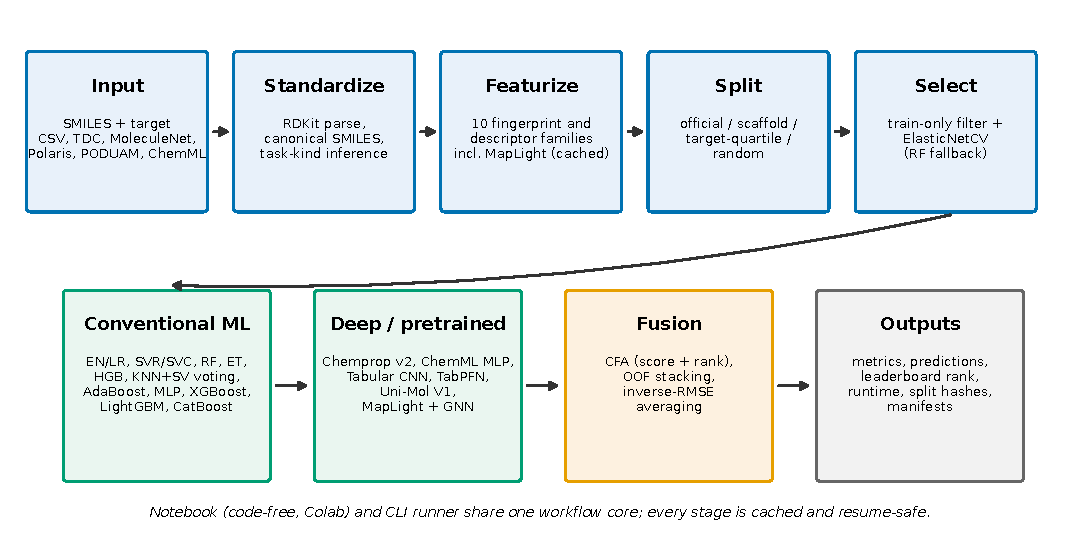
\includegraphics[width=\textwidth]{figures/figure1_workflow.pdf}
\caption{The QSARena workflow. Data ingestion and standardization, featurization, splitting and train-only feature selection are followed by a model library spanning conventional machine learning, deep and pretrained models, and fusion; every stage writes cached, resumable artifacts. The code-free notebook and the command-line runner share this core.}
\label{fig:workflow}
\end{figure}

For each dataset the runner builds molecular features, applies the train/test split and train-only feature selection, fits the conventional, deep and pretrained models, fuses and ensembles their predictions, and writes cross-dataset performance tables; optional families are skipped when their dependencies, hardware or dataset-size guardrails are unmet, so the rest of a run continues.

\subsection{Datasets and curation}\label{sec:datasets}

Benchmark datasets were drawn from five public collections through dedicated loaders: ChemML bundled examples \cite{haghighatlari2020chemml}; TDC single-prediction ADME and Tox tasks \cite{huang2021tdc}; MoleculeNet physicochemical datasets (ESOL \cite{delaney2004esol}, FreeSolv \cite{mobley2014freesolv}, Lipophilicity); Polaris ADME benchmarks; and the PODUAM point-of-departure datasets \cite{vonborries2026uncertainty}. Each dataset is represented internally by a specification recording the SMILES column, target column, recommended split, recommended metric, benchmark suite and any leaderboard reference metadata.

Before featurization, targets were coerced to numeric, rows with missing or non-finite SMILES or targets were removed, and each SMILES was parsed with RDKit \cite{rdkit} and re-encoded as canonical SMILES, molecules that failed to parse being dropped. Targets from the TDC, MoleculeNet, Polaris, literature and PFAS auxiliary suites kept their native scale, and other datasets were log10-transformed when all target values were positive (Additional file~2, Section~4.2).

For TDC datasets, the official \texttt{admet\_group} train/test split was used wherever PyTDC provides one. This distinction matters for interpretation and we preserve it throughout: 22 TDC datasets and 5 Polaris datasets used official predefined splits, while the remaining 17 used locally generated scaffold, random or target-quartile splits and are therefore \emph{not} directly leaderboard-equivalent (Section~\ref{sec:leaderboard}). Task kind was inferred from the targets rather than from catalog metadata, strict binary 0/1 targets being routed to classification, so four binary datasets that the dataset catalog listed with a regression metric when the benchmark ran (corrected since) are analysed as classification throughout.

\subsection{Molecular representations}\label{sec:representations}

Ten RDKit feature families were computed, and all ten were used: Morgan \cite{rogers2010ecfp}, ECFP6 and FCFP6 circular fingerprints; RDKit path, layered, atom-pair and topological-torsion fingerprints; MACCS keys \cite{durant2002maccs}; the RDKit 2D descriptor set; and the ``MapLight classic'' composite of the MapLight TDC submission \cite{notwell2023admet} --- Morgan and Avalon count fingerprints \cite{gedeck2006qsar}, the extended reduced graph (ErG) pharmacophore fingerprint \cite{stiefl2006erg} and about 200 RDKit descriptors --- which the feature-selection analyses report as its three components (\texttt{avalon}, \texttt{erg} and the \texttt{maplight} descriptor panel). Bit widths, matrix finalization and the content-addressed feature store are described in Additional file~2, Section~4.3 and Additional file~1, Note~S2.

\subsection{Splitting and cross-validation}\label{sec:splitting}

Each dataset used one of four split strategies: its official predefined partition where one exists (any molecule present in both partitions being reassigned by SMILES), a Bemis--Murcko scaffold split \cite{bemis1996properties} that assigns whole scaffold groups to the test set, a target-quartile split (the runner's default) or a random split, with a test fraction of 0.2 and random seed 13. Cross-validation folds mirrored the split geometry (scaffold groups, quartile bins or random folds), and feature selection was nested inside them (Section~\ref{sec:selection}); procedures and fallbacks are given in Additional file~2, Section~4.4.

\subsection{Feature filtering and selection}\label{sec:selection}

A pre-filter fitted on the training partition only removed near-constant, near-uniform binary and duplicate columns, and a cross-validated elastic net, also fitted on training rows only, then kept the features with non-negligible coefficients, capped at 10\% of the training-row count, falling back to random-forest importance ranking when it exceeded a wall-clock limit (default 7,200\,s) or failed (thresholds and grids in Additional file~2, Section~4.5 and Additional file~1, Note~S2). Because that limit makes the selection depend on the speed of the machine (see Limitations), the runner also has a deterministic selection mode, which removes the limit, runs the selector single-threaded and can load a previously deposited selection; the A100 selection used for every result in this paper is deposited with the artifacts.

% META:methods_nested_selection
\textbf{Feature selection inside cross-validation.} Selecting features on the whole training split and then cross-validating models on the selected columns lets every held-out fold influence the selection, which inflates cross-validated scores. Selection was therefore refitted inside every cross-validation fold, on that fold's training rows only and with the method pinned to the one recorded for the full training split. These fold-specific selections produce both the cross-validated metrics of every model that uses the selected features and their out-of-fold ensemble predictions (Section~\ref{sec:lineage}); Section~\ref{sec:nestedcv} reports the bias they remove. Where TabPFN's local fold refits did not fit the GPU, its cross-validated scores are withdrawn rather than reported from the leaky protocol.
% /META

\subsection{Model library}\label{sec:models}

The 31 models fall into eight families (Table~\ref{tab:families}): conventional machine learning (scikit-learn \cite{pedregosa2011scikit}, XGBoost \cite{chen2016xgboost} and CatBoost \cite{prokhorenkova2018catboost} estimators, a compact tabular convolutional network and a leaderboard-parity MapLight CatBoost \cite{notwell2023admet}); two ChemML multilayer perceptrons (deep tabular); MapLight\,+\,GNN, which fits CatBoost on MapLight classic features plus pretrained graph isomorphism network (GIN) embeddings; five Chemprop v2 graph neural networks \cite{yang2019analyzing,heid2024chemprop,graff2026chempropv2}, each trained as a three-model ensemble; the 3D pretrained Uni-Mol V1 and V2 \cite{zhou2023unimol,ji2024unimol2}; the tabular foundation model TabPFN \cite{hollmann2023tabpfn}; combinatorial fusion; and stacking and averaging ensembles. Every hyperparameter was fixed in advance; each model's settings and per-dataset availability are listed in Additional file~1, Note~S2 and Table~S12, and the options in Additional file~2, Sections~4.6 and~4.8. One conventional model, XGBoost on the full, unselected ADMETboost feature set (MACCS, ECFP4 and PubChem fingerprints, Mol2Vec embeddings, and Mordred and RDKit 2D descriptors), bypasses feature selection; it joined the library after the main run (Section~\ref{sec:lineage}; Additional file~1, Note~S3). An optional genetic-algorithm tuning stage was disabled throughout, so no GA-tuned model appears in any result and its value is untested here.

\subsection{Combinatorial fusion and ensembling}\label{sec:fusion}

Combinatorial fusion analysis (CFA) \cite{hsu2006combinatorial} combined the best model of each workflow in score and rank space, choosing among equal, performance-weighted and diversity-weighted combinations by training metric. Three ensembles were built over the same prediction pool: out-of-fold stacking with a RidgeCV meta-model (logistic for classification), a weighted average with weights proportional to each member's inverse out-of-fold error, and a simple average (Additional file~2, Sections~4.9--4.10; Additional file~1, Note~S2). Member selection, filtering, weighting and the stacking meta-model read only out-of-fold predictions on the training split (Section~\ref{sec:lineage}); held-out test predictions are never consulted. Regression member predictions are clipped to the range of the training targets before they are combined, so that a member which extrapolates wildly on a few molecules cannot dominate; this uses no test-split labels. CFA outputs and members without out-of-fold predictions are excluded, as is TabPFN, because most of its full-fit predictions came from the Prior Labs API while its fold refits used the local package.

\subsection{Evaluation metrics}\label{sec:metrics}

Every model's regression (RMSE, mean absolute error, $R^2$, Spearman correlation) or classification (AUROC, AUPRC, balanced accuracy, Matthews correlation coefficient) metrics are written out. Cross-dataset ranking used RMSE for regression and, for classification, each dataset's TDC-designated primary metric (AUPRC on five CYP datasets, AUROC otherwise); comparisons against published leaderboards re-select the best model under the leaderboard's own metric, which is MAE or Spearman for several TDC regression tasks, and both are reported (Additional file~2, Section~4.12; Additional file~1, Tables~S1 and~S7). Because absolute differences are not comparable across target units --- an RMSE gap of 1.0 is negligible for hepatocyte clearance and fatal for log-solubility --- every cross-dataset summary of closeness to the per-dataset best uses the \textbf{relative} gap $|\text{score}-\text{best}|/|\text{best}|$.

\subsection{Leaderboard comparison}\label{sec:lbmethod}

Where curated leaderboard references existed, the best QSARena model was compared against published values whose metric matched the dataset's leaderboard metric, giving the gap to the top-1 reference, the gap to the top-10 cutoff and an estimated rank among the published entries. Reference rows were aggregated from TDC, MoleculeNet and Polaris leaderboards together with a manually curated set of TDC ADMET reference values and, for ESOL and Lipophilicity, current literature values in place of the 2017-era MoleculeNet baselines.

Three limits of this procedure should be kept in view. First, ``estimated rank'' reflects the references available for a dataset, not a live leaderboard submission; a dataset with few references yields an optimistic-looking rank. Second, ranks are only leaderboard-equivalent where the split protocol matches, which is true for the 22 TDC \texttt{admet\_group} datasets and the 5 Polaris datasets but not for the 10 comparable datasets evaluated on locally generated splits. Third, the published values include self-reported ranks from different dates and entries with documented leakage (Sections~\ref{sec:leaderboard} and~\ref{sec:platforms}). We therefore treat every estimated rank as a provisional, secondary analysis.

\subsection{Model selection protocols}\label{sec:protocols}

We report every headline result under two selection protocols.

\paragraph{Test-selected.} The best model per dataset is the one with the best held-out primary metric. This is the protocol used by AutoML leaderboard submissions generally, and it is what Sections~\ref{sec:nowinner}--\ref{sec:consistency} and the first half of Section~\ref{sec:leaderboard} report for comparability with published entries.

\paragraph{Cross-validation-selected.} The model is chosen per dataset solely by its cross-validated primary metric on the training partition, and its held-out score is then read off without further choice. This estimates what a practitioner obtains when the test set is genuinely untouched. It is available for the models that emit cross-validated metrics --- the conventional estimators, TabPFN and the ChemML MLPs --- but not for Chemprop, Uni-Mol, MapLight\,+\,GNN or the fusion methods, so it is a conservative lower bound on what a fully CV-driven QSARena would achieve. Its cross-validated scores come from feature selection refitted inside each fold (Section~\ref{sec:selection}).

\subsection{Reproducibility and computing environment}\label{sec:environment}

Runs are resumable: completed datasets and compatible intermediates are reused, and each run records a configuration signature, per-dataset status manifests, split-signature hashes, per-stage runtimes and a SHA-256 manifest of its artifacts (Additional file~2, Sections~6 and~9).

The base benchmark ran on NSF ACCESS Jetstream2 \cite{hancock2021jetstream2,boerner2023access} on one NVIDIA A100-SXM4-40GB GPU with 32 CPU cores under Linux, in fp32 precision; the device inventory and configuration are recorded with the deposited artifacts, and the wall-clock and cost figures in this paper come from that run. All figures, tables and quoted numbers regenerate from the deposited artifacts with one command, which also writes a machine-readable record of every headline number, and a companion script fails if the manuscript text and the artifacts disagree. Per-molecule prediction files are excluded from the repository for size, so prediction-level diagnostics such as inter-model prediction diversity cannot be reproduced from it alone; they are included in the archived release (see Availability of data and materials).

\subsection{Benchmark runs and ensemble reconstruction}\label{sec:lineage}

The reported results combine three runs that share one data, split, feature and feature-selection configuration, verified through stage signatures: the base benchmark; a repair run that trained only what a Chemprop harness fault and a disabled TabPFN had left missing; and a rebuild of every ensemble from out-of-fold predictions, with feature selection nested inside each cross-validation fold (Section~\ref{sec:selection}). No base model was retrained, except that ten conventional and gradient-boosting models were refitted with probability outputs on four binary datasets on which they had saved hard class labels, and TabPFN's label-based results on three of those datasets were withdrawn; the descriptor model of Section~\ref{sec:models} joined the library after an exploratory analysis, which can flatter test-selected comparisons (Section~\ref{sec:nowinner} bounds its effect). Additional file~1, Note~S1 gives the full account.

\subsection{Use of large language models}\label{sec:llm}

Large language model (LLM) assistants were used during software development, analysis and manuscript preparation; as the journal requires, that use is documented here. Anthropic's Claude models (Claude Sonnet 4.6, Claude Opus 5 and Claude Opus 5.5), accessed through the Claude Code coding assistant, were used to (i) write, refactor, test and debug parts of the QSARena code base and its test suite; (ii) write and run analysis scripts, monitor long-running benchmark jobs and diagnose their failures; and (iii) draft and edit manuscript text and supplementary documentation. Human Chemical was also used. The author specified the study design, the benchmark protocol and every analytical decision, reviewed and validated all AI-assisted code and text, and takes full responsibility for the content. No LLM is an author. LLMs did not generate data or results: every reported number is computed by scripted pipelines from the benchmark artifacts and checked against them automatically, and the code is covered by unit, integration and tutorial tests. All figures, including the graphical abstract, are rendered by code directly from benchmark outputs; no AI image-generation tools were used.

\section{Results and discussion}\label{sec:results}

\subsection{Benchmark coverage}\label{sec:coverage}

We executed QSARena across 44 datasets under a single fixed configuration (full model profile, random seed 13, Chemprop seed 42). They comprise 22 regression and 22 classification tasks drawn from five collections: TDC (32), Polaris ADME (5), MoleculeNet (3), ChemML (2) and PODUAM (2). They span 280 to 13,445 molecules (median 1,605; 156,052 in total) and four split protocols (27 predefined, 12 scaffold, 4 target-quartile, 1 random). Thirty-one models produced at least one valid result, yielding 1094 valid model--dataset evaluations. The dataset catalog, with each dataset's estimated leaderboard rank and the best published value it is measured against, is given in Additional file~1, Table~S6. A 45th dataset, \texttt{tdc\_herg\_central}, was abandoned for compute budget after more than 24 hours without completing, and \texttt{polaris\_adme\_fang\_hppb\_1}, interrupted in the base run, was completed by the repair run (Additional file~1, Note~S1).

\subsection{No single model family dominates}\label{sec:nowinner}

Consistent with the cross-suite studies cited in the Introduction, no single model family won across the benchmark (Fig.~\ref{fig:wins}, Table~\ref{tab:families}). Stacking and averaging ensembles built from the other families produced the most outright wins (22 of 44 datasets: 14 regression, 8 classification), followed by conventional machine learning (6), Chemprop v2 and the 3D pretrained Uni-Mol models (5 each), TabPFN (3), the MapLight\,+\,GNN descriptor--graph hybrid (2, both regression), combinatorial fusion (1) and deep tabular networks (0). No single model family won more than 14\% (6 of 44). The ensemble row is not a like-for-like competitor: ensembles are built \emph{from} the other families' predictions, although their member selection and weights use only out-of-fold predictions, so the row estimates what the pipeline can obtain from honest training-set predictions rather than what stacking can gain by consulting the final test set.

Three of conventional machine learning's six wins come from the descriptor model added after the main run (Section~\ref{sec:lineage}). With that model removed as a candidate, conventional machine learning wins 3 datasets, the ensembles 24 and Uni-Mol 6, and no single family wins more than 6 (Additional file~1, Table~S14); the ensemble rows still contain it as a member, so this bounds only its direct effect. The 3D pretrained family won two classification datasets as well as three regression datasets (aqueous solubility, microsomal clearance and half-life, properties for which conformational and shape information is mechanistically plausible as signal), so conformer-based pretraining is not a regression-only tool; under the shorter training schedule of our earlier consumer-GPU run it won no classification dataset (Section~\ref{sec:hardware}).

\begin{figure}[htbp]
\centering
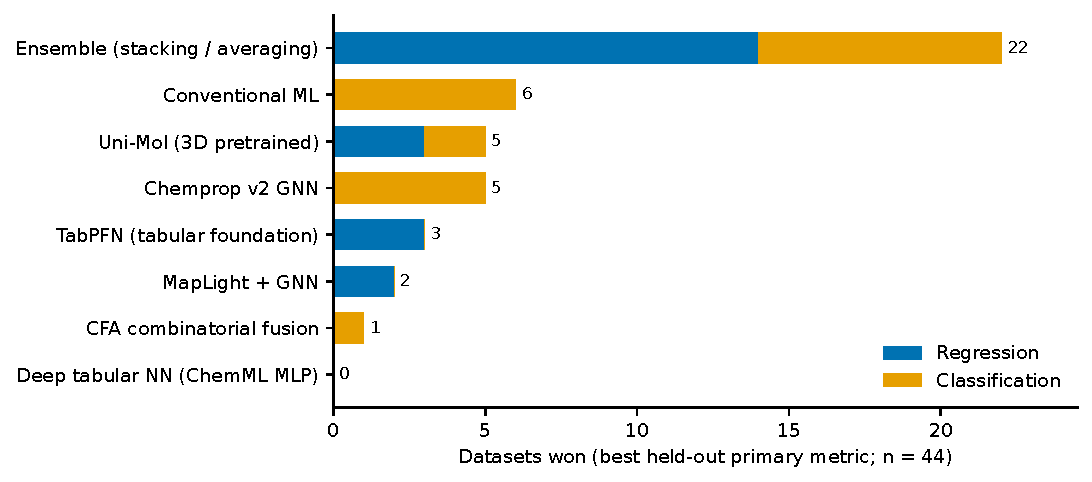
\includegraphics[width=0.85\textwidth]{figures/figure2_wins_by_family.pdf}
\caption{Datasets won by each model family, split by task kind. A win is the best held-out primary metric on that dataset among all 31 models. \emph{Single split and single seed: individual placements are provisional and no variance is estimated (see Limitations).}}
\label{fig:wins}
\end{figure}

Per-dataset winners, with the corresponding cross-validation-selected model, are listed in Additional file~1, Table~S1, and every family's gap to the best on every dataset is shown in Additional file~1, Figure~S5. These are single-split, single-seed outcomes: an unknown fraction of individual winners would change under a different seed, so we read Fig.~\ref{fig:wins} as a distribution of capability across families and base the claim on that breadth (see Limitations).

\subsection{Consistency versus peak performance}\label{sec:consistency}

Win counts reward only the single best model per dataset, so Table~\ref{tab:families} also reports, for each family, the median relative gap to the per-dataset best, the share of datasets on which the family's best member came within 5\% of the best result, and that member's median rank.

\begin{landscape}
\begin{table}[htbp]
\centering
\scriptsize
\caption{Model-family coverage and consistency. Gaps are relative to the per-dataset best primary metric. ``Within 5\% of best'' counts datasets where the family's best member fell within 5\% of the dataset winner. Families evaluated on fewer than 44 datasets were limited by task applicability, size guardrails or backend failures (Additional file~1, Table~S4); their percentages are computed over the datasets on which they ran. All values derive from a single split and seed, so adjacent rows are not separated (see Limitations).}
\label{tab:families}
\begin{tabularx}{\linewidth}{@{}>{\raggedright\arraybackslash}Xrrrrrrrr@{}}
\toprule
\textbf{Model family} & \textbf{Models} & \makecell[r]{\textbf{Datasets}\\\textbf{with}\\\textbf{valid}\\\textbf{results}} & \makecell[r]{\textbf{Wins}\\\textbf{(regression)}} & \makecell[r]{\textbf{Wins}\\\textbf{(classification)}} & \makecell[r]{\textbf{Median}\\\textbf{gap to}\\\textbf{best,}\\\textbf{regression}\\\textbf{(\%)}} & \makecell[r]{\textbf{Median}\\\textbf{gap to}\\\textbf{best,}\\\textbf{classification}\\\textbf{(\%)}} & \makecell[r]{\textbf{Within}\\\textbf{5\% of}\\\textbf{best (\%}\\\textbf{of}\\\textbf{datasets)}} & \makecell[r]{\textbf{Median}\\\textbf{rank of}\\\textbf{family-best}\\\textbf{model}} \\
\midrule
Ensemble (stacking /\allowbreak{} averaging) & 2 & 44 & 6 & 7 & 4.3 & 2.2 & 61.4 & 3.0 \\
Uni-\allowbreak{}Mol (3D pretrained) & 2 & 44 & 4 & 4 & 5.2 & 2.2 & 56.8 & 4.0 \\
Chemprop v2 GNN & 5 & 42 & 3 & 5 & 7.8 & 2.7 & 54.8 & 6.0 \\
TabPFN (tabular foundation) & 2 & 44 & 4 & 1 & 6.9 & 15.3 & 29.5 & 10.0 \\
Conventional ML & 15 & 44 & 1 & 3 & 3.8 & 4.1 & 59.1 & 4.0 \\
Map\allowbreak{}Light + GNN & 1 & 44 & 4 & 0 & 8.0 & 12.8 & 27.3 & 12.0 \\
CFA combinatorial fusion & 1 & 38 & 0 & 2 & 8.5 & 2.3 & 42.1 & 6.0 \\
Deep tabular NN (ChemML MLP) & 2 & 44 & 0 & 0 & 20.5 & 9.7 & 18.2 & 16.0 \\
\bottomrule
\end{tabularx}
\end{table}
\end{landscape}


The out-of-fold ensembles were the most consistent (within 5\% of the best on 84\% of datasets) and conventional machine learning the most consistent single family (66\%); every other family was within 5\% on at most half of the datasets. Two cautions apply. Families with more models have more chances to produce a near-best member, so the 16-model conventional family is flattered relative to single-model families; and the ensemble row is not a like-for-like competitor, as noted above. Section~\ref{sec:components} quantifies how much the fusion layer actually adds.

Uneven coverage does not drive these orderings. Chemprop v2 produced valid results on 38 to 42 of the 44 datasets depending on variant, TabPFN on 41 and Uni-Mol V2 on 17 (Section~\ref{sec:failures}). Restricted to the 41 datasets on which all eight families produced a result, the single families keep their win counts (conventional machine learning 6, Chemprop and Uni-Mol 5 each, TabPFN 3), the ensembles win 19, and conventional machine learning keeps the smallest median gap of any single family (3.7\%, against 5.8\% for Uni-Mol and 5.9\% for Chemprop); on the 17 datasets on which Uni-Mol V2 ran, Uni-Mol wins 4 and conventional machine learning 2 (Additional file~1, Table~S13). The comparison between conventional and pretrained families therefore does not depend on which datasets each family covered.

% META:results_nested_selection
\subsection{Nested feature selection removes most cross-validation optimism}\label{sec:nestedcv}

Fitting feature selection once on the whole training split and then cross-validating on the selected columns lets every validation fold help choose its own features. A controlled comparison on 9 datasets, with identical features, models and folds and selection fitted either outside or inside the folds, isolated this effect: fitting selection outside the folds raised the overstatement of cross-validated over test RMSE by a median of 22.7 percentage points for ElasticNetCV, 6.1 for random forest and 2.5 for SVR, and raised it in 26 of 27 dataset-model pairs (sign test, p < 0.001).

Across the benchmark, on datasets with predefined or scaffold test splits, nesting the selection (Section~\ref{sec:selection}) cut the median overstatement of cross-validated over test scores from 15.9\% to 3.4\% across 462 model-dataset pairs (lower in 96\% of them). That is the level shown by fixed-configuration models trained without feature selection on the same folds (3.4\%), so the optimism that remains reflects the gap between training-set folds and harder held-out splits rather than leakage (see Limitations). Test-set results are unchanged by construction: the deployed models and their selected features are the same. The correction matters in two places downstream. The cross-validation-selected protocol of Section~\ref{sec:leaderboard} now rests on unbiased cross-validated scores, and the out-of-fold ensembles no longer over-weight members whose fold predictions benefited from the leak.
% /META

Nesting the selection also changed the ensembles, because the leak had inflated the out-of-fold predictions of members that use selected features and the stacker over-weighted them. It improved the best ensemble on 39 of the 44 datasets (median error reduction 4.9\% for regression; median AUROC gain 0.7\% for classification), while no base model's test result changed. Under the out-of-fold protocol with nested feature selection, ensembles won 22 datasets (14 regression, 8 classification), against 16 (7 and 9) under the leaky first protocol and 12 (6 and 6) when their out-of-fold predictions came from the outer feature selection (Additional file~1, Note~S1).

\subsection{Leaderboard competitiveness, and the cost of honest model selection}\label{sec:leaderboard}

This section reports two kinds of result: the comparison between selection protocols, which is internal to a single run and is the primary result, and estimated ranks against published values, which are provisional because the reference set contains entries with documented leakage and each rank rests on one split and seed.

Across the leaderboard-comparison layer, 37 datasets could be compared against 430 published reference values. The best QSARena model per dataset placed within the estimated top ten on 35 of 37 datasets, with a median estimated rank of 3 and six estimated first places (Additional file~1, Table~S7). The two datasets below the top ten, Tox21 and skin reaction, were both evaluated on locally generated scaffold splits that are harder than the references they are scored against.

\begin{figure}[htbp]
\centering
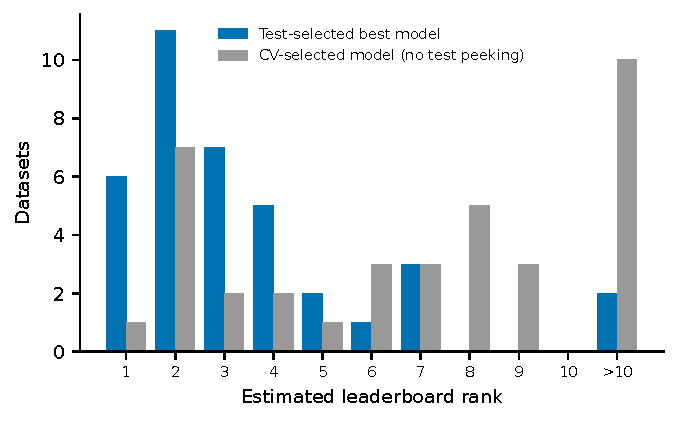
\includegraphics[width=0.62\textwidth]{figures/figure3_leaderboard_rank.pdf}
\caption{Estimated leaderboard placement across 37 comparable datasets: distribution of estimated ranks for the test-selected best model and for the model selected by cross-validation alone. Per-dataset ranks are shown in Additional file~1, Figure~S4. \emph{Single split and single seed: individual placements are provisional and no variance is estimated (see Limitations).}}
\label{fig:rank}
\end{figure}

Comparability varies by dataset, and the aggregate obscures it. Restricted to the 22 TDC datasets evaluated on official \texttt{admet\_group} splits --- the only subset directly comparable to the public TDC leaderboard --- the test-selected model placed in the top ten on \textbf{all 22}, with a median rank of 2.5 and two estimated first places. On the 5 Polaris datasets it placed in the top ten on all 5, median rank 4, with one first place. The remaining 10 comparable datasets used locally generated splits and are \emph{not} leaderboard-equivalent; both sub-top-ten results and three of the six first places fall in this group, and those should be read as ``competitive with published values under a comparable but not identical protocol'', not as leaderboard claims. Table~\ref{tab:leaderboardsummary} gives the breakdown by comparison class.

\begin{table}[htbp]
\centering
\footnotesize
\caption{Rank among curated published reference values, by comparison class. Only the 27 datasets with official predefined splits --- 22 TDC ADMET Benchmark Group and 5 Polaris ADME --- are directly comparable to a public leaderboard; the remaining 10 are scored against published values under a comparable but not identical protocol and are reported separately rather than pooled. Columns: ``n'' is the number of datasets in the class; ``test'' selects the best model per dataset on held-out data; ``CV'' selects by cross-validation only. Per-dataset detail is in Additional file~1, Table~S7. Single split and single seed, so individual placements are provisional.}
\label{tab:leaderboardsummary}
\begin{tabularx}{\textwidth}{@{}>{\raggedright\arraybackslash}Xrrrrr@{}}
\toprule
\textbf{Comparison class} & \textbf{n} & \textbf{Top-10 test} & \textbf{Median rank test} & \textbf{Top-10 CV} & \textbf{Median rank CV} \\
\midrule
TDC ADMET Group (official) & 22 & 22 & 2.5 & 16 & 7.0 \\
Polaris ADME (official) & 5 & 5 & 4.0 & 4 & 6.0 \\
Local splits (not leaderboard-\allowbreak{}equivalent) & 10 & 8 & 2.5 & 7 & 8.5 \\
All comparable datasets & 37 & 35 & 3.0 & 27 & 7.0 \\
\bottomrule
\end{tabularx}
\end{table}


That headline, however, is produced by choosing the best of 31 models using held-out scores. Under the stricter protocol in which the model is chosen by cross-validation alone (Section~\ref{sec:protocols}), top-ten placement falls from 35 to 27 of 37 datasets, first places from six to one, and the median estimated rank from 3 to 7 (Fig.~\ref{fig:rank}). On the official TDC subset the fall is from 22 of 22 to 16 of 22. Across all 44 datasets, the cross-validation-selected model was the overall winner on 4 datasets and sat a median of 7.7\% above the per-dataset best.

\textbf{That eight-dataset gap has two causes, and separating them changes its interpretation.} Cross-validation selection is restricted to models that emit cross-validated metrics, which in this run excludes Chemprop, the Uni-Mol models, MapLight\,+\,GNN and the fusion methods. The comparison above therefore confounds the cost of not peeking at the test set with the cost of losing those candidate families. To separate them we added a third protocol that holds the candidate set fixed at the cross-validation-eligible models and selects among them on the test metric:

% tabularx against \linewidth, not a fixed tabular: sn-jnl's text block is 372.0pt, far narrower
% than the article-class proof's 472.3pt, and the fixed version overflowed it by 59.5pt.
\begin{center}
\begin{tabularx}{\linewidth}{@{}>{\raggedright\arraybackslash}X>{\raggedright\arraybackslash}Xccc@{}}
\toprule
Selection & Candidate set & \makecell{Top\\ten} & \makecell{First\\places} & \makecell{Median\\rank} \\
\midrule
Test metric & Full 31-model library & 35/37 & 5 & 3 \\
Test metric & CV-eligible models only & 28/37 & 3 & 5 \\
Cross-validation & CV-eligible models only & 27/37 & 1 & 7 \\
\bottomrule
\end{tabularx}
\end{center}

Read down the table, \textbf{7 of the 8 lost placements come from narrowing the candidate set and 1 from honest selection}; the median rank moves from 3 to 5 on library breadth and from 5 to 7 on selection protocol. The breadth of the model library is therefore the strongest available argument for running many model families rather than one well-tuned architecture. The cost of honest model selection is smaller but still visible: within the cross-validation-eligible pool it reduces estimated first places from 3 to 1.

The individual ranks in Fig.~\ref{fig:rank} carry unquantified seed variance, but the shift is large and one-sided, and it would take implausibly favourable seed variance to erase an eight-dataset gap. Any leaderboard entry that selects among candidate models or configurations using test-set feedback carries the same inflation, and a reproducibility audit of the TDC leaderboard \cite{koleiev2026critical} suggests that such selection is rarely documented. We take the cross-validation-selected result --- top ten on nearly three-quarters of comparable datasets --- as the honest estimate of what a practitioner should expect, and a conservative one, since Chemprop, Uni-Mol, MapLight\,+\,GNN and the fusion methods were ineligible for it.

\textbf{The reference set is itself imperfect.} The same audit found that only three top-ranked TDC ADMET entries --- CaliciBoost, MapLight and MapLight\,+\,GNN --- passed all reproducibility and leakage checks, and reported data leakage in several others, so our cross-validation-selected model is ranked against a population that includes entries inflated by the very selection effect measured here. The gap between our two protocols, internal to one run and free of this contamination, is the more trustworthy quantity, and future leaderboard-relative claims should be scored against an audit-verified subset once one is maintained.

For ESOL and Lipophilicity we scored against current literature values rather than the dated MoleculeNet leaderboard; the Lipophilicity first place is a nominal margin of 0.001 RMSE, well inside single-split variance, and we make no state-of-the-art claim for either.

\subsection{What the pipeline's components contribute}\label{sec:components}

Because fusion and ensembling add computational cost and interpretive complexity, we asked what each layer of the pipeline actually buys (Table~\ref{tab:ensemble}).

\begin{landscape}
\begin{table}[htbp]
\centering
\scriptsize
\caption{Ensemble and fusion value-add against the best single base model available on the same dataset, under each dataset's primary metric.}
\label{tab:ensemble}
\begin{tabularx}{\linewidth}{@{}>{\raggedright\arraybackslash\hsize=1.000\hsize}X>{\raggedright\arraybackslash\hsize=1.000\hsize}Xrrrrrrr@{}}
\toprule
\textbf{Fusion method} & \textbf{Task} & \textbf{Datasets} & \textbf{Overall wins} & \textbf{Top-3} & \textbf{Beats best base} & \makecell[r]{\textbf{Loses to}\\\textbf{best base}} & \textbf{Median rank} & \makecell[r]{\textbf{Median}\\\textbf{rel.}\\\textbf{change vs}\\\textbf{best base}} \\
\midrule
OOF stacking & classification & 22 & 8 & 9 & 8 & 14 & 4.000 & -\allowbreak{}0.016 \\
Other ensemble & classification & 22 & 0 & 8 & 6 & 16 & 6.000 & -\allowbreak{}0.030 \\
CFA fusion & classification & 16 & 2 & 6 & 2 & 14 & 4.000 & -\allowbreak{}0.023 \\
CFA fusion & regression & 22 & 0 & 4 & 1 & 21 & 8.500 & -\allowbreak{}0.075 \\
OOF stacking & regression & 22 & 1 & 2 & 1 & 21 & 10.500 & -\allowbreak{}0.127 \\
Other ensemble & regression & 22 & 0 & 2 & 0 & 22 & 8.000 & -\allowbreak{}0.084 \\
\bottomrule
\end{tabularx}
\end{table}
\end{landscape}


Taking the best fusion method per dataset, some fusion beat the best single model on 9 of 22 classification datasets, with a median relative improvement of 1.4\% where it won, and on 14 of 22 regression datasets, with a median improvement of 4.1\% where it won. Across all datasets the typical fusion result was better than the best single model for regression (median $+3.2$\%) and slightly worse for classification (median $-0.3$\%), because fusion also loses where it does not win, so fusion is worth its cost on most regression datasets and on roughly two classification datasets in five. These margins, median relative changes below 3\% on a single split and seed, are the most fragile quantities we report.

A staged ablation over the same artifacts (Additional file~1, Table~S2) agrees: starting from conventional machine learning alone, adding MapLight classic features improved the achievable result on 9 of 44 datasets, adding the neural and pretrained backends improved 26, adding CFA improved 6, and adding the out-of-fold ensemble layer improved 22. The deep and pretrained backends are therefore the largest single source of incremental accuracy, which cuts against a purely ``conventional models are enough'' reading of Fig.~\ref{fig:wins}, but that accuracy is not free (Section~\ref{sec:cost}) and does not make any pretrained family a reliable default.

\subsection{Feature representations}\label{sec:features}

We quantified which representation families the leak-free elastic-net selector actually retained, relative to a uniform-selection baseline (Fig.~\ref{fig:features}; Additional file~1, Table~S3). Of 12,137 selected features across all datasets, the three components of the MapLight classic composite accounted for 46.2\%, against 22.9\% of the available feature pool --- a clear enrichment for the composite as a whole.

\begin{figure}[htbp]
\centering
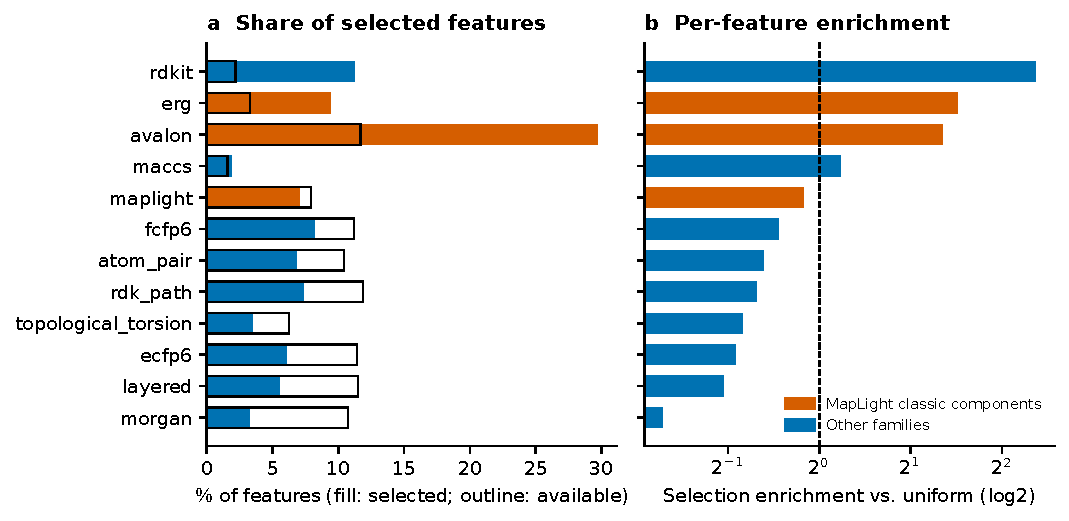
\includegraphics[width=\textwidth]{figures/figure4_feature_family_enrichment.pdf}
\caption{Feature-family representation among selected features. (a) Share of selected features (filled) against share of available features (outlined). (b) Per-feature selection enrichment relative to a uniform baseline, $\log_2$ scale. Components of the MapLight classic composite are highlighted.}
\label{fig:features}
\end{figure}

On a per-feature basis the ordering is more informative. The compact RDKit 2D descriptor panel was by far the most enriched family ($5.16\times$ uniform), followed by ErG ($2.86\times$) and Avalon ($2.54\times$); MACCS keys were marginally enriched ($1.18\times$); and the large hashed circular and path fingerprints were all \emph{de}-enriched, including FCFP6 ($0.73\times$). A few hundred interpretable descriptors thus earn selection far above their numerical weight, and thousands of hashed fingerprint bits below theirs (Avalon's large absolute share, 29.7\% of selected features, reflects its size as much as its per-feature value), so for practitioners with limited compute the RDKit descriptor panel plus one compact pharmacophore representation captures most of the selectable signal. This is consistent with representation benchmarks reporting that descriptor sets outperform fingerprints as standalone representations \cite{kamuntavicius2025benchmarking} and that fixed representations lead on most datasets \cite{deng2023systematic}.

\subsection{Computational cost}\label{sec:cost}

The complete benchmark consumed 111.8 hours of recorded wall-clock time across 44 datasets on the A100 node (median 1.89\,h per dataset; maximum 11.2\,h for the 13,445-molecule hERG-Karim set). Per-model cost is each model's own incremental wall-clock time; fusion methods are also charged the summed cost of the base-model pool they consume, since a fusion result cannot be obtained without it.

\begin{figure}[htbp]
\centering
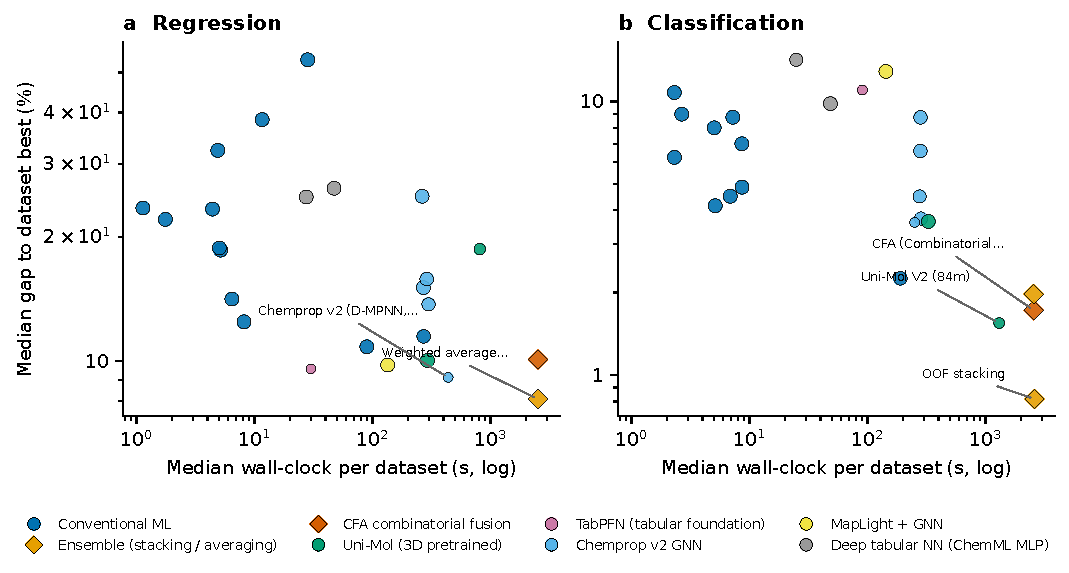
\includegraphics[width=\textwidth]{figures/figure5_cost_vs_value.pdf}
\caption{Median wall-clock time per dataset against median relative gap to the per-dataset best, by model, separately for regression (a) and classification (b). Both axes are logarithmic; diamonds mark fusion methods, which are charged the summed cost of the base-model pool they consume in addition to their own, since a fusion result cannot be obtained without it.}
\label{fig:cost}
\end{figure}

Per-family median cost spans more than three orders of magnitude (Table~\ref{tab:cost}): 0.3\,s for CFA and 0.6\,s for the ensemble meta-models (excluding their base pool), 6.8\,s for conventional machine learning, 39.8\,s for the deep tabular networks, 137\,s for MapLight\,+\,GNN, 269\,s for Chemprop v2 and 374\,s for the Uni-Mol models. The 3D pretrained family therefore costs roughly 55 times the median conventional model per dataset, in exchange for 5 wins and a family median rank of 6.5: a deliberate trade, not a default. The models that won most datasets --- gradient-boosted trees and the linear meta-models over them --- carry no pretraining corpus at all, unlike the published comparators MolE and MolGPS \cite{mendezlucio2024mole,sypetkowski2024molgps}; their sizes, per-model costs and feature-selection scaling are given in Additional file~1, Note~S6 and Table~S16.

\begin{table}[htbp]
\centering
\scriptsize
\setlength{\tabcolsep}{3pt}
\caption{Per-family computational cost and model size in this benchmark. Wall-clock times are each model's own incremental time per dataset on the A100 run hardware; fusion and ensemble methods are also given with the summed cost of the base-model pool they consume. Published comparators are in Additional file~1, Table~S16.}
\label{tab:cost}
\begin{tabularx}{\textwidth}{@{}>{\raggedright\arraybackslash\hsize=1.170\hsize}Xrr>{\raggedright\arraybackslash\hsize=0.830\hsize}Xrr@{}}
\toprule
\textbf{Model family} & \makecell[r]{\textbf{Fits}\\\textbf{timed}} & \makecell[r]{\textbf{Median}\\\textbf{own}\\\textbf{wall-clock}\\\textbf{(s)}} & \textbf{IQR own wall-clock (s)} & \makecell[r]{\textbf{Median}\\\textbf{incl.}\\\textbf{base}\\\textbf{pool}\\\textbf{(s)}} & \makecell[r]{\textbf{Median}\\\textbf{trainable}\\\textbf{parameters}} \\
\midrule
CFA combinatorial fusion & 44.0 & 0.3 & 0-\allowbreak{}0 & 1,378 &  \\
Ensemble (stacking /\allowbreak{} averaging) & 87.0 & 0.6 & 0-\allowbreak{}1 & 1,378 &  \\
Conventional ML & 440.0 & 6.8 & 3-\allowbreak{}20 &  & 157,953 \\
Deep tabular NN (ChemML MLP) & 88.0 & 39.8 & 27-\allowbreak{}94 &  & 90,369 \\
Map\allowbreak{}Light + GNN & 44.0 & 137.4 & 126-\allowbreak{}160 &  &  \\
Chemprop v2 GNN & 25.0 & 268.6 & 229-\allowbreak{}274 &  & 325,552 \\
Uni-\allowbreak{}Mol (3D pretrained) & 61.0 & 373.5 & 170-\allowbreak{}1285 &  & 47,331,652 \\
\bottomrule
\end{tabularx}
\end{table}


\subsection{Model coverage and backend failures}\label{sec:failures}

Not every model ran on every dataset, and we report the gaps rather than silently analysing only successes (Additional file~1, Table~S4 and Note~S6): beyond task applicability, Uni-Mol V2 produced valid results on 17 of 44 datasets at 84\,M parameters and none at 164\,M or 310\,M, Chemprop v2 on 38 to 42 per variant, and TabPFN was withdrawn on three large binary datasets (Section~\ref{sec:lineage}). Restricting the comparison to the datasets covered by every family leaves it unchanged (Section~\ref{sec:consistency}), and Additional file~1, Figure~S5 shows every family's gap on every dataset.

\subsection{Hardware sensitivity: datacentre GPU versus consumer laptop GPU}\label{sec:hardware}

Because accessibility is a central claim of this work, we compared the A100 run with an earlier execution of the same benchmark on a consumer laptop GPU (NVIDIA GeForce RTX 4060 Laptop GPU, Windows, cost-optimized model profile) under identical analysis code. On the 37 datasets with byte-identical held-out partitions, verified by split-signature hash, the best single model (ensembles and fusion excluded, because the two runs built them under different protocols) changed the primary metric by a median of $+0.50$\% --- the A100 run was better on 22 datasets and the consumer-GPU run on 13 --- so at this resolution the two hardware configurations are indistinguishable in accuracy. The A100 bought capacity rather than accuracy (a broader model profile, longer Chemprop and Uni-Mol schedules, Uni-Mol V2 and a complete run in 112 rather than 155 hours), and those changes, not the hardware class, explain the shifts in which family wins, most notably Uni-Mol's classification wins. Neither the selection-protocol result nor the estimated placements depend on datacentre hardware (Additional file~1, Table~S5 and Note~S6).

\subsection{Effort required of the user}\label{sec:effort}

Two properties of the benchmark design bear directly on what a practitioner should expect. First, \textbf{every number in this paper was produced under a single fixed configuration}: the same profile, seeds, feature families, selector and model library were applied to all 44 datasets, spanning five suites, two task types and a 48-fold range of dataset size, with no bespoke feature engineering, model choice or hyperparameter tuning for any dataset. The results therefore estimate what a single run on a new dataset yields; an expert tuning campaign might do better, and the honest counterpart remains the cross-validation-selected protocol of Section~\ref{sec:leaderboard}. Second, \textbf{obtaining that result requires no local installation or hardware}: the notebook runs end-to-end in Google Colab on the free tier, where the user supplies a CSV of SMILES and targets and selects columns through form widgets, and Section~\ref{sec:hardware} shows that accuracy does not depend on the class of hardware underneath.

These claims have limits: the configuration was informed by our own earlier development on overlapping datasets, so it is not a blind default in the strictest sense, and datasets far outside the sampled size and endpoint range may need more attention, while unusual splits, custom featurization or new backends need the command-line interface and a local environment.

\subsection{Comparison with existing automated QSAR platforms}\label{sec:platforms}

The automated QSAR systems closest to QSARena in purpose are QSAR Workbench \cite{cox2013qsarworkbench}, which generates hundreds of descriptor\,$\times$\,learner\,$\times$\,split models but leaves the choice among them to human judgement, the step QSARena automates and then audits; the closed-source commercial Schr\"odinger AutoQSAR and DeepAutoQSAR \cite{dixon2016autoqsar,schrodinger2024deepautoqsar}, whose published TDC benchmark ranks DeepAutoQSAR against two named comparators rather than on the leaderboard; and MetaQSAR \cite{ambure2026metaqsar}, a free desktop application with classical learners and OECD-aligned applicability-domain methods. QSARena is free and runnable without installation, backed by a deposited artifact trail with a script that fails if the text and the artifacts disagree, and evaluated on five suites rather than one; the others offer professional support or regulatory case studies that it lacks (Additional file~1, Note~S5 and Table~S15). ADMET-AI \cite{swanson2024admetai} is not one of the 31 models evaluated here: our \texttt{Chemprop v2 (D-MPNN + RDKit2D)} variant reimplements its Chemprop-RDKit recipe through Chemprop v2 and produced valid results on 38 of 44 datasets, so parity with ADMET-AI is untested, and we ran no head-to-head comparison against it or any other system.

\textbf{Where QSARena does not lead.} Published rankings are usually each paper's rank at its own publication date (our curated reference table contains 64 rows claiming first place across 28 datasets), so we re-scored all reference values jointly, after correcting three that were on the wrong scale. MaxQsaring, which reports first place on 19 of 22 TDC tasks \cite{xu2025maxqsaring}, then holds 7 first places but is top-3 on 19 of 22 with a median rank of 2, the strongest system in the reference set; ADMETboost's reported 18 first places \cite{tian2022admetboost} fall to zero, because it has been overtaken on all 22 datasets since 2022. Against that corrected reference set, QSARena's best model per dataset reaches a median rank of 2.5 on the 22 official TDC tasks under test-based selection, and falls to a median rank of 7 under cross-validation-only selection (Section~\ref{sec:leaderboard}). MaxQsaring's median rank of 2 is therefore better than ours under either protocol, and we make no claim to accuracy leadership.

\subsection{Regulatory alignment with the OECD (Q)SAR principles}\label{sec:oecd}

The OECD validation principles ask for a defined endpoint, an unambiguous algorithm, a defined applicability domain, appropriate measures of goodness of fit, robustness and predictivity, and, where possible, a mechanistic interpretation \cite{oecd2004principles}; the OECD (Q)SAR Assessment Framework turns them into a structured reliability check for individual predictions \cite{oecd2023qaf}. QSARena records what such an audit needs: dataset and split provenance for the endpoint; the full run configuration and environment manifests for the algorithm; per-prediction domain labels for the applicability domain; training, cross-validated and held-out metrics for fit, robustness and predictivity; and model-specific feature attributions, or an explicit ``not available'' status, for interpretation.

To test the third and fourth principles, a supplementary reliability study on the 22 official TDC ADMET splits (Additional file~1, Table~S8) fitted one fixed reference model, a random forest on Morgan radius-2 fingerprints plus RDKit 2D descriptors with 20\% of each training partition reserved for conformal calibration; it is not the per-dataset selected QSARena model and it is not a multi-seed result. Structural applicability-domain flags were weak. Roy's descriptor-standardization rule \cite{roy2015applicability} covered a median of 95.7\% of test compounds (range 92.6--99.5\%) but separated higher out-of-domain error on only 8 of 17 evaluable datasets (median out/in error ratio 0.91; 34.8\% higher outside the domain for regression); a k-nearest-neighbour Tanimoto domain covered 89.7\%, with higher out-of-domain error on 13 of 21 (ratio 1.15, 15.3\% higher); and requiring both to agree gave 87.0\% coverage and higher error on 14 of 22 (7.9\% higher). Prediction-reliability flags were much stronger: low-confidence predictions (conformal interval width for regression, posterior-probability margin for classification) covered a median of 51.2\% of test compounds and had higher error on all 22 datasets (median ratio 3.30; 230.3\% higher, 108.0\% for regression and 382.1\% for classification). Split-conformal calibration was close to its nominal 90\% target (regression interval coverage 93.2\%, classification prediction-set coverage 90.9\%; median classifier ECE 0.065, Brier score 0.137). The workflow therefore emits what an OECD-style audit needs, and reliability signals identify high-error predictions, but structural domain flags barely separate error on these splits and the audit covers a reference model rather than the selected ones.

% META:section_meta_summary
\subsection{When does each family win?}\label{sec:meta}

A dataset-property meta-analysis, a form of per-dataset algorithm selection from dataset meta-features~\cite{olier2018metaqsar}, asked whether properties of the dataset alone predict which family comes close to the best. It was exploratory and, at n = 44, inconclusive: 1 of 48 family $\times$ meta-feature correlations survived Benjamini--Hochberg control, a leave-one-dataset-out depth-3 decision tree predicted the best family group with balanced accuracy 0.32 against 0.25 for the majority class (permutation p = 0.138), and a pre-registered regret-based selector did not reliably beat always choosing the family with the best average record (permutation p = 0.099). The per-dataset winner therefore remains an empirical question, which is the case for benchmarking many families on every dataset (Additional file 1, Note S4, Figures~S1--S3 and Tables S9--S11).
% /META

\section{Limitations}\label{sec:limitations}

\paragraph{Single split and single seed: the principal limitation of this work.} Every result reported here derives from one split and one random seed per dataset, whereas the TDC convention is to report mean\,$\pm$\,standard deviation over five independent seeds; we treat this as a deliberate scope boundary of the study. Multi-seed evaluation over the official TDC splits is implemented in the runner but was never executed for this benchmark: in the base run the stage was scheduled to run after all datasets finished, and that run was interrupted before reaching it. A five-seed replication of the full benchmark was in any case beyond the available budget: the single-seed run alone consumed 112 hours of A100 time (Section~\ref{sec:cost}), implying roughly 560 hours.

We report no variance estimates or significance tests for model-to-model comparisons, so we cannot distinguish a genuine difference between two models from seed-to-seed noise: (i) each per-dataset winner is the winner \emph{on this split}, and the win counts are a coarse distribution across families; (ii) adjacent rows of Table~\ref{tab:families}, such as CFA, Uni-Mol and Chemprop at 48 to 50\% within 5\% of best, are not separated; (iii) the ensemble and fusion margins of Section~\ref{sec:components} (median relative changes below 3\%) are the results most vulnerable to seed variance; and (iv) estimated leaderboard ranks inherit the same instability. The hardware comparison gives an empirical sense of the noise floor: across the 37 datasets with identical splits, changing the entire execution environment moved the best single-model score by a median of $+0.50$\% (Section~\ref{sec:hardware}), so differences between models smaller than roughly a percent should not be interpreted.

Three results do not rest on close margins and should survive this limitation: no single model family won more than 6 of 44 datasets; the model-selection gap is large enough to change the leaderboard interpretation; and the cost differences in Table~\ref{tab:cost} span orders of magnitude. The estimated top-ten placements are less secure, because they also depend on the quality of the published reference set, which seed replication would not fix. Every specific model-to-model comparison here is provisional pending multi-seed replication, the necessary next step for this work and the first thing a user should run on a dataset that matters to them.

\textbf{Model selection.} As quantified in Section~\ref{sec:leaderboard}, the test-selected headline is an optimistic maximum over 31 models. The cross-validation-selected protocol is the honest comparator but is itself incomplete, since the Chemprop, Uni-Mol, MapLight\,+\,GNN and fusion families do not emit cross-validated metrics in this run.

% META:limitation_cvleak
\textbf{Residual cross-validation optimism.} With feature selection nested inside the folds (Section~\ref{sec:selection}), cross-validated scores still exceed the corresponding test scores by a median of 3.4\% on datasets with predefined or scaffold test splits (per-model medians $-$3.9\% to 6.5\% across 19 CV-scored models). Fixed-configuration models that select no features show 3.4\% on the same folds, so the remainder reflects the gap between training-set folds and harder held-out splits rather than leakage. The cross-validation-selected protocol in Section~\ref{sec:leaderboard} should be read with that margin in mind.
% /META

\paragraph{Self-benchmarking asymmetry.} Competitors were not re-run under our pipeline, so every leaderboard comparison sets our single controlled run against other groups' best published effort; the bias runs against us where a published entry reflects tuning we did not perform and in our favour where it was itself selected on test data, and its net direction is unknown.

\paragraph{Estimated ranks are not submissions.} Ranks are computed against curated reference values of varying density (2 to 30 references per dataset), not by submission to a live leaderboard, and are a provisional secondary analysis (Section~\ref{sec:lbmethod}).

\paragraph{Incomplete backend coverage.} Chemprop is incomplete on several datasets, the two larger Uni-Mol V2 variants produced no valid results, and TabPFN is withdrawn on three datasets, so Fig.~\ref{fig:wins} is not a fully balanced tournament (Section~\ref{sec:failures}), although restricting the comparison to the datasets every family covered leaves it unchanged (Section~\ref{sec:consistency}).

\paragraph{Feature selection is not reproducible across machines by default.} ElasticNetCV feature selection falls back to random-forest importance after its 7,200-second limit, and which datasets reach the limit depends on the hardware. Re-running selection on the RTX 4060 workstation changed the selected features on 6 of the 44 datasets (Tox21, Ames, LD50, ESOL, CYP2C9 and AqSolDB). Every reported model, and the ensemble rebuild, uses the selection from the A100 run, which is deposited with the artifacts; the runner's deterministic selection mode can load it, or remove the time limit for new runs (Section~\ref{sec:selection}).

\paragraph{One target per task.} Multi-label datasets (Tox21, ToxCast) were reduced to a single label, so results on those datasets are not comparable to multi-task leaderboard entries.

\paragraph{Applicability domain and calibration.} The diagnostics of Section~\ref{sec:oecd} describe a fixed reference random forest, not the selected models, so regulatory use should run the reliability workflow on the final chosen model and dataset.

% META:limitation_meta
\textbf{Meta-analysis.} The meta-analysis (Section~\ref{sec:meta}; Additional file 1, Note S4) relates dataset properties to family performance, but it inherits the single-split, single-seed design: individual winners are noisy, which is why it models the continuous gap and bootstraps over datasets, not seeds. With n = 44 datasets the meta-models are kept to four predictors, and the diversity and similarity features depend on the fingerprint used (the ECFP6 sensitivity check preserved the sign of 92\% of the fingerprint-dependent correlations). How informative similarity-based domain metrics are itself varies with training-set diversity~\cite{sheridan2015relative}.
% /META

\section{Conclusions}\label{sec:conclusions}

Across 44 molecular property benchmarks from five suites, evaluated under one leakage-controlled pipeline and one fixed configuration, the clearest lessons are about how models are selected and compared, not about which single model is best. Nested, train-only feature selection cut median cross-validation optimism from 15.9\% to 3.4\%, and decomposing the gap between test-selected and cross-validation-selected leaderboard standing shows that most of it --- 7 of 8 top-ten placements --- comes from the breadth of the candidate library and only 1 from selecting on held-out rather than cross-validated data, an inflation that applies to any comparably selected entry but is rarely reported. Consistent with recent cross-suite reports, no model family dominated: out-of-fold ensembles over the other families won the most datasets (22 of 44) and were the most consistent, no single family won more than 6, and conventional machine learning was the most consistent single family. Compact descriptors --- the RDKit 2D panel and pharmacophore fingerprints --- were selected far above their numerical share, and large hashed fingerprints below theirs. Genetic-algorithm tuning was disabled throughout, so its value is untested here. We encourage leaderboard entries to report both selection protocols, together with the candidate set each one saw.

Every number above came from one configuration, with no per-dataset feature engineering, architecture choice or hyperparameter tuning, and from a single split and seed, so conclusions that rest on close margins are provisional. Repeating the benchmark on a consumer laptop GPU moved the best single-model score by a median of $+0.50$\% across identically split datasets, and the code-free notebook runs in Google Colab with no installation (Section~\ref{sec:effort}). For practitioners who can run only one configuration, our results support a specific default: a MapLight-style descriptor panel with gradient-boosted trees, ensembled by inverse-error averaging, adding a 3D pretrained model where the compute budget allows and the endpoint plausibly depends on molecular shape.



\section*{Declarations}

\bmhead{Ethics approval and consent to participate}
Not applicable.

\bmhead{Consent for publication}
Not applicable.

\bmhead{Availability of data and materials}
\textbf{Software availability.}
\begin{description}
\item[Project name:] QSARena
\item[Project home page:] \url{https://github.com/ScottCoffin/QSARena}
\item[Operating system(s):] Platform independent (Windows, macOS, Linux, Google Colab)
\item[Programming language:] Python 3.11
\item[Installation:] \texttt{pip install qsarena} (console scripts \texttt{qsarena-benchmark}, \texttt{qsarena-applicability-domain} and \texttt{qsarena-examples}), or clone the repository and run the scripts directly; the code-free notebook requires no installation at all and runs in Google Colab. A step-by-step installation and usage tutorial, in which every command is executed by an automated test on bundled example data, is provided as Additional file~2
\item[Other requirements:] RDKit, scikit-learn, pandas, NumPy, SciPy, joblib, PyYAML; heavy backends are optional extras (\texttt{qsarena[boosting]}, \texttt{[deep]}, \texttt{[graph]}, \texttt{[foundation]}, \texttt{[notebook]}). Exact versions for reproducing the benchmark are pinned in \texttt{requirements-cpu.txt} / \texttt{requirements-cuda.txt} and the conda environment files, which should be used in preference to the pip extras for exact reproduction
\item[License:] MIT License (OSI-approved); see the \texttt{LICENSE} file in the repository
\item[Any restrictions to use by non-academics:] None beyond the repository license
\end{description}

The QSARena source code, benchmark runner, analysis notebook and the complete benchmark artifacts analysed in this study are available in the QSARena repository, \url{https://github.com/ScottCoffin/QSARena}. The repository contains the workflow core (\texttt{qsar\_workflow\_core.py}), the notebook builder, the command-line benchmark runner (\texttt{run\_qsarena\_benchmarks.py}, installed as the \texttt{qsarena-benchmark} console script), the dataset registry, the curated leaderboard reference tables, the per-dataset benchmark artifacts (metrics, selected features, selector coefficients, split-signature hashes, runtime records, fusion candidate tables and ensemble weights) for the run from which every reported result is computed (\texttt{benchmark\_results/qsarena\_benchmark\_oof\_ensemble/}) and for the runs it was built from (\texttt{benchmark\_results/autoqsar\_benchmark\_20260623\_153839/} and \texttt{benchmark\_results/qsarena\_benchmark\_chemprop\_fixed/}) together with the consumer-GPU (RTX 4060 laptop) comparison run of Section~\ref{sec:hardware}, whose directory is named in Additional file~1, Note~S1, the post-hoc feature-expansion analysis of Additional file~1, Note~S3 (\texttt{benchmark\_results/qsarena\_feature\_expansion/}), the analysis notebook (\texttt{portable\_colab\_qsar\_bundle/benchmark\_results\_summary.ipynb}), and the scripts that regenerate every figure, table and quoted number in this paper (\texttt{render\_manuscript\_assets.py}, \texttt{verify\_manuscript\_numbers.py}). Pinned conda and pip environment specifications, an Apptainer container definition and Slurm/OpenStack submission scripts are included for independent re-execution.

The datasets analysed during the current study are available in the following public repositories: the Therapeutics Data Commons ADMET Benchmark Group and single-prediction tasks, via PyTDC (\url{https://tdcommons.ai}) \cite{huang2021tdc}; the MoleculeNet ESOL \cite{delaney2004esol}, FreeSolv \cite{mobley2014freesolv} and Lipophilicity (ChEMBL deposition CHEMBL3301361, \url{https://doi.org/10.6019/CHEMBL3301361}) \cite{astrazeneca2015chembl} datasets, as distributed by MoleculeNet \cite{wu2018moleculenet}; the Polaris ADME benchmarks (\url{https://polarishub.io}) \cite{ash2025polaris,wognum2025polarissoftware}, derived from the Biogen ADME dataset \cite{fang2023adme}; the PODUAM point-of-departure datasets (\url{https://github.com/kejbo/PODUAM}) \cite{vonborries2026uncertainty}; and the ChemML example datasets \cite{haghighatlari2020chemml}. Each dataset's source, version and split are recorded in the dataset registry and in Additional file~1, Table~S6.

No registration or login is needed to download, install or run QSARena, so reviewers can test it anonymously. The optional Google Colab path requires a Google account; the same notebook also runs in any local Jupyter installation, and Additional file~2 covers local installation step by step.

A versioned release archived on Zenodo, including the per-molecule prediction files excluded from the repository for size, will be deposited before publication and its DOI cited here.
% TODO(author): mint Zenodo DOI and replace this sentence. The deposit is staged: .zenodo.json and CITATION.cff hold the
% metadata, and dist/zenodo/ holds the two per-molecule prediction archives with sha256 manifests (re-verified against
% the repository files on 2026-10-06; ZENODO.md gives the steps).

\bmhead{Competing interests}
The author declares no competing interests.

\bmhead{Funding}
This work was supported by the California Office of Environmental Health Hazard Assessment (OEHHA). Computing resources for the benchmark were provided in kind through NSF ACCESS allocation CIS261142 on Jetstream2 (see Acknowledgements). The funders had no role in study design, data collection and analysis, decision to publish, or preparation of the manuscript.

\bmhead{Authors' contributions}
SC conceived the study, developed the software, designed and executed the benchmark, analysed the results and wrote the manuscript. The author read and approved the final manuscript.

\bmhead{Acknowledgements}
This work used Jetstream2 GPU at Indiana University through allocation CIS261142 from the Advanced Cyberinfrastructure Coordination Ecosystem: Services \& Support (ACCESS) program, which is supported by U.S. National Science Foundation grants \#2138259, \#2138286, \#2138307, \#2137603, and \#2138296 \cite{boerner2023access}. Jetstream2 \cite{hancock2021jetstream2} is supported by the National Science Foundation under Grant 2005506. Any opinions, findings, and conclusions or recommendations expressed in this material are those of the author and do not necessarily reflect the views of the National Science Foundation.

The views expressed are those of the author and do not necessarily represent those of the California Environmental Protection Agency or the Office of Environmental Health Hazard Assessment.
% TODO(author): confirm the required OEHHA/CalEPA disclaimer wording.


\bibliography{references}

\end{document}
